%
% $RCSfile: framework.tex,v $
%
% Copyright (c) 2001-2004. Christian Heller. All rights reserved.
%
% Permission is granted to copy, distribute and/or modify this document
% under the terms of the GNU Free Documentation License, Version 1.1
% or any later version published by the Free Software Foundation;
% with no Invariant Sections, with no Front-Cover Texts and with no Back-Cover
% Texts. A copy of the license is included in the section entitled
% "GNU Free Documentation License".
%
% http://www.cybop.net
% - Cybernetics Oriented Programming -
%
% http://www.resmedicinae.org
% - Information in Medicine -
%
% @author Christian Heller <christian.heller@tuxtax.de>
% @author Jens Bohl <info@jens-bohl.de>
%

\section{CYBOP}
\label{cybop_heading}

Section \ref{design_principles_heading} introduced essential design patterns
that represent the main structure of the CYBOP framework. Section
\ref{an_extended_component_lifecycle_heading} explained the Component Lifecycle
and section \ref{ontology_heading} the well-known idea of ontology. Now these
design principles and concepts will be combined to comprise their advantages and
to increase the demanded quality characteristics: high flexibility and
maintainability.\\
\emph{Structure by Hierarchy} -- this is the basic idea behind CYBOP. While this
principle has been applied to many domain and knowledge models, especially in the
field of \emph{Artificial Intelligence} (AI), it apparently has not been used
for the design of systems yet.\\
Let us recall the \emph{Model View Controller} design pattern which is used in
one or another form by a majority of systems, today. There is a \emph{View} which
mostly is a \emph{Graphical User Interface} (GUI). It consists of for example a
frame, panel, menubar and smaller components which are all part of the frame's
hierarchy. Then, there is the \emph{Controller}. The \emph{Hierarchical MVC}
pattern suggested to use a controller hierarchy consisting of \emph{MVC Triads}.
Finally, there is the \emph{Model}. Not only AI systems use a \emph{Hierarchy}
to structure their domain data. The OpenEHR project \cite{openehr} does the same.\\
Reflecting these facts, one question is at hand: \emph{If View, Controller and
Model ideally have a hierarchical structure, why not creating whole software
systems after this paradigm?} Isn't every system essentially a \emph{Tree} of
objects?\\
Extending the concept of \emph{Hierarchical Model View Controller} to whole
software architectures, CYBOP was designed to be the domain-independent backbone
for information systems of any kind. Originally designed for medical purposes,
it should also become usable for insurance, financial or other standard
applications in future.

\subsection{Class Item}
\label{class_item_heading}

As shown, tree-like structures can be realized by the \emph{Composite} pattern.
In CYBOP, this pattern can be found simplified in class {\tt Item}
(figure \ref{class_item_figure}) which is super type of all other classes.
References, respectively relations to child elements are held within a hashmap.
No attributes are used except of this hashmap. Every element of the map can be
accessed by a special key value.

\begin{figure}[ht]
    \begin{center}
       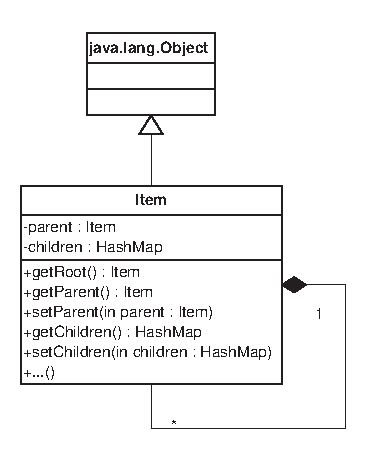
\includegraphics[scale=0.8]{eps/item.eps}
       \caption{Class Item}
       \label{class_item_figure}
    \end{center}
\end{figure}

But that also means that any particular \texttt{set}- and \texttt{get}-methods
become superfluous. The recommendation to encapsulate attributes produces thousands
of lines of code whose usefulness is at least questionnable. In probably 90\% of
cases, the \texttt{set} and \texttt{get} methods consist of only one single line
accessing an attribute value. Sometimes, additional lines with an update function
for other parts of the system are added. They are called whenever an attribute
value is changed by a \texttt{set} method:

\begin{verbatim}
public void setValue(Type v) {

    this.value = v;
    getUpdateManager().update(this);
}
\end{verbatim}

But this update notification could as well be taken over by the parent object
that was calling the \texttt{set} method on one of its child objects:

\begin{verbatim}
public void method() {

    child.setValue(v);
    getUpdateManager().update(child);
}
\end{verbatim}

In the end, the responsibility of encapsulation falls to the super class
\emph{Item} with its access methods, alone. It is the only remaining container
class in the whole framework. No other container classes have to be written ever.
For the issue of sorting children (such as to simulate a \emph{List}), other
concepts have to be used which are partly unclear yet and will not be described
further in this paper.\\
Another advantage of having just one container class is that the unpredictable
behaviour in object oriented languages, when inheriting a container (hashtable)
can be avoided. Find more details in \cite{javaiaq}.\\
Finally, there is the issue of security. If a system's security manager is
forwarded in the \emph{globalize} lifecycle method from object to object, as
described in section \ref{an_extended_component_lifecycle_heading}, then it can
be stored as one child of the \emph{Item} super class. Whenever a child needs
to be accessed, a parent's security manager can check for permittance.

\subsection{Basic Structure}
\label{basic_structure_heading}

Comprising the design patterns \emph{Composite}, \emph{Layers}, and
\emph{Chain of Responsibility}, the CYBOP framework is comparable to a big tree
containing objects organized in different levels. These levels are determined by
a special \emph{System Ontology} (as opposed to a \emph{Knowledge Ontology} like
for example OpenEHR \cite{openehr}) and might become the topic of a follow-up
paper. Figure \ref{basic_structure_figure} shows the object tree and the different
levels of granularity.

\begin{figure}[ht]
    \begin{center}
       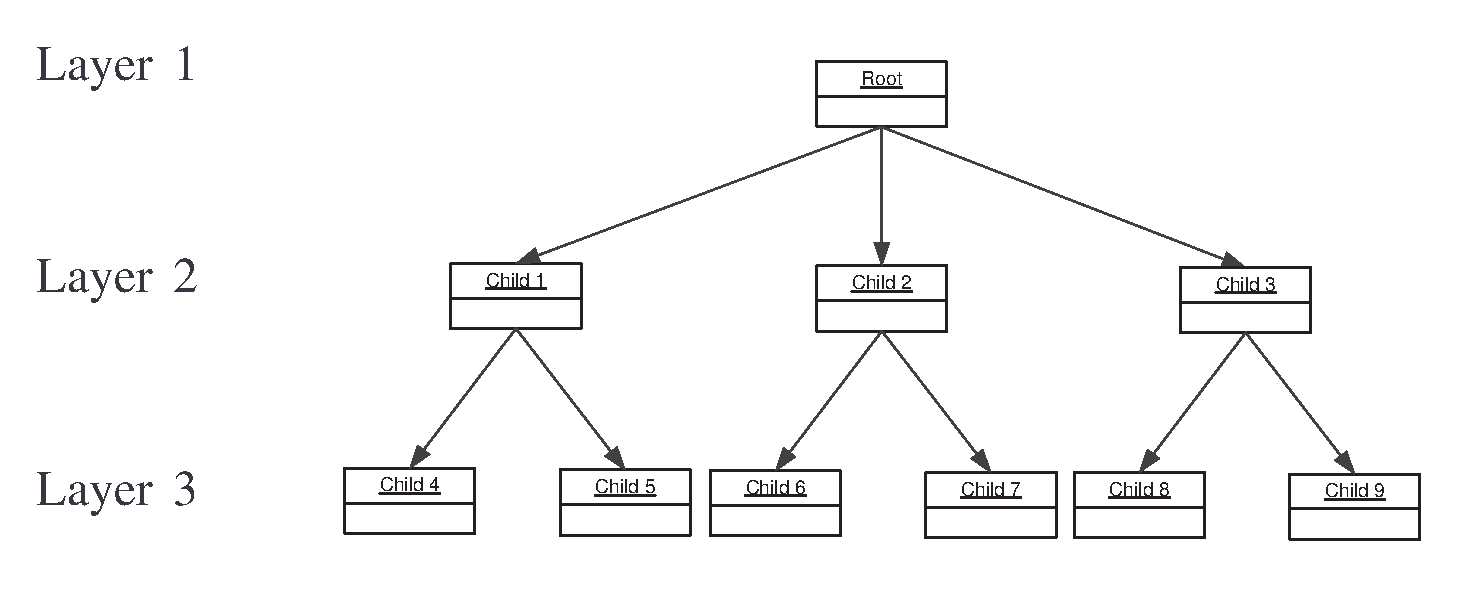
\includegraphics[scale=0.3]{eps/framework-structure.eps}
       \caption{Basic Structure}
       \label{basic_structure_figure}
    \end{center}
\end{figure}

